
\de{ĐỀ THI GIỮA HỌC KỲ II NĂM HỌC 2022-2023}{THPT Nguyễn Hữu Cảnh}


\begin{bt}%[0T7B1-2]%[Đề GHKII 2022-2023, TheHung Nguyen]%[Thpt Nguyễn Hữu Cảnh]
	Xét dấu biểu thức $f(x)=2x^2-x-15$.
	\loigiai{Ta có $f(x)=0\Leftrightarrow 2x^2-x-15=0\Leftrightarrow \hoac{& x=3 \\ & x=-\dfrac{5}{2}.} $\\
		Bảng xét dấu
		\begin{center}
			
\begin{tikzpicture}
				\tkzTabInit[lgt=1.2,espcl=2.5,deltacl=0.6]
				{$x$/1,$f(x)$/1}{$-\infty$,$-\dfrac{5}{3}$,$3$,$+\infty$}
				\tkzTabLine{,+,0,-,0,+,}				
			\end{tikzpicture}
		\end{center}
	Dựa vào bảng xét dấu
	\begin{itemize}
		\item $f(x)=0$ tại $x=-\dfrac{5}{3}$ và $x=3$.
		\item	$f(x)\le 0 $ khi $x\in  \left[-\dfrac{5}{3};3\right]$.
		\item $f(x)> 0 $ khi $x\in\left(-\infty ;-\dfrac{5}{3}\right)\cup(3 ;+\infty)$.
	\end{itemize}
	}
\end{bt}

\begin{bt}%[0T7B1-2]%[Đề GHKII 2022-2023, TheHung Nguyen]%[Thpt Nguyễn Hữu Cảnh]
	Tìm các giá trị của $m$ để bất phương trình $x^2-(m+2) x+5 m+1>0$ luôn đúng với mọi $x \in \mathbb{R}$.
	\loigiai{Ta có 
		\begin{eqnarray*}
			& & x^2-(m+2) x+5 m+1>0,\quad \forall x \in \mathbb{R}\\
			&\Leftrightarrow & \heva{& a>0 \\ & \Delta \le 0}\\
			&\Leftrightarrow & (m+2)^2-4(5m+1)\le 0\\
			&\Leftrightarrow &m^2-16m\le 0\\
			&\Leftrightarrow & 0\le m\le 16.
		\end{eqnarray*}
	Vậy $0\le m\le 16$ thì thỏa yêu cầu bài toán.
	}
\end{bt}

\begin{bt}%[0T7B2-1]%[Đề GHKII 2022-2023, TheHung Nguyen]%[Thpt Nguyễn Hữu Cảnh]
	Giải bất phương trình $-2x^2+3x+5 \leq 0$.
	\loigiai{Ta có $-2 x^2+3 x+5 = 0\Leftrightarrow \hoac{& x=-1 \\ & x=\dfrac{5}{2}.}$\\
	Bảng xét dấu 
		\begin{center}
		\begin{tikzpicture}
			\tkzTabInit[lgt=3,espcl=2.5,deltacl=0.6]
			{$x$/1,$-2x^2+3x+5$/1}{$-\infty$,$-1$,$\dfrac{5}{2}$,$+\infty$}
			\tkzTabLine{,-,0,+,0,-,}				
		\end{tikzpicture}
	\end{center}	
	Dựa vào bảng xét dấu 	$-2x^2+3x+5 \leq 0\Leftrightarrow x\in \left(-\infty; -1\right]\cup\left[\dfrac 52; +\infty\right)$.\\
	Vậy $S=\left(-\infty; -1\right]\cup\left[\dfrac 52; +\infty\right)$.
	}
\end{bt}

\begin{bt}%[0T7B2-2]%[Đề GHKII 2022-2023, TheHung Nguyen]%[Thpt Nguyễn Hữu Cảnh]
	Anh An dùng $60$ m lưới rào quanh một mảnh vườn hình chữ nhật đề trồng rau. Biết rằng một cạnh theo chiều dài vườn là một bức tường (nên không cần rào), do đó anh An chi cần rào ba cạnh còn lại của hình chữ nhật để làm vườn. Giả sử diện tích mành vườn không nhỏ hơn $400$m$^2$. Hỏi chiều rộng của mảnh vườn có giá trị nhỏ nhất là bao nhiêu?
	\loigiai{Gọi $x$ là chiều rộng của mảnh vườn hình chữ nhật, (đơn vị là mét). Điều kiện $x>0$.\\
		Khi đó chiều dài phải rào của khu vườn là $60-2x$. \\
		Vì diện tích khu vườn không nhỏ hơn $400$ m$^2$ nên ta có
		$$x(60-2x)\ge 400\Leftrightarrow -2x^2+60x-400\ge 0\Leftrightarrow 10\le x\le 20.$$
		Vậy chiều rộng của vườn cần có giá trị nhỏ nhất là $10$ m.
	}
\end{bt}


\begin{bt}%[0T7B3-2]%[Dự án đề kiểm tra GHKII NH22-23- Nguyễn Văn Sang]%[THPT Nguyễn Hữu Cảnh]
	Giải phương trình $2 \sqrt{x^2-x-1}=\sqrt{x^2+2 x+5}$.
\loigiai{
Bình phương  hai vế phương trình  $2 \sqrt{x^2-x-1}=\sqrt{x^2+2 x+5}\quad(*)$, ta được 
\begin{eqnarray*}
	&&2 \sqrt{x^2-x-1}=\sqrt{x^2+2 x+5}\\
	&\Rightarrow& 4 \left( x^2-x-1\right) =x^2+2 x+5\\
	&\Leftrightarrow& 3x^2-6x-9=0\\
	&\Leftrightarrow&\hoac{& x=-1\\ & x=3.}
\end{eqnarray*}
Thử lại
\begin{itemize}
	\item Với $x=-1$, thay vào $(*)$ thoả nên $x=-1$ nhận.
	\item Với $x=3$, thay vào $(*)$ thoả nên $x=3$ nhận.
\end{itemize}
Vậy tập nghiệm của phương trình là $S=\left\lbrace-1;3\right\rbrace$.
}
\end{bt}

\begin{bt}%[0T9B1-1]%[Dự án đề kiểm tra GHKII NH22-23- Nguyễn Văn Sang]%[THPT Nguyễn Hữu Cảnh]
	Trong mặt phẳng $Oxy$, cho tam giác $ABC$ có $A(1;3)$, $B(3;5)$, $C(4;2)$.
	\begin{enumerate}
		\item Tìm tọa độ trung điểm $M$ của cạnh $AB$ và tọa độ trọng tâm $G$ của tam giác $ABC$.
		\item Chứng minh tam giác $ABC$ cân và tính chu vi tam giác $ABC$.
	\end{enumerate}
	\loigiai{
	\begin{enumerate}
		\item Tìm tọa độ trung điểm $M$ của cạnh $AB$ và tọa độ trọng tâm $G$ của tam giác $ABC$.
		\begin{itemize}
			\item Vì $M$ là trung điểm $AB$ ta có
			$\heva{& x_M=\dfrac{x_A+x_B}{2}=2 \\ & y_M=\dfrac{y_A+y_B}{2}=4.}$\\
			Vậy $M(2;4)$.
			\item Vì $G$ là trọng tâm tam giác $ABC$ ta có
			$\heva{& x_G=\dfrac{x_A+x_B+x_C}{3}=\dfrac{8}{3} \\ & y_G=\dfrac{y_A+y_B+y_C}{3}=\dfrac{10}{3}.}$\\
			Vậy $G\left(\dfrac{8}{3};\dfrac{10}{3}\right) $.
		\end{itemize}
		\item Chứng minh tam giác $ABC$ cân và tính chu vi tam giác $ABC$.\\
		Ta có
		\begin{itemize}
			\item $\overrightarrow{AB}=(2;2)\Rightarrow AB=2\sqrt{2}$.
			\item $\overrightarrow{AC}=(3;-1)\Rightarrow AC=\sqrt{10}$.
			\item $\overrightarrow{BC}=(1;-3)\Rightarrow BC=\sqrt{10}$.
		\end{itemize}
		Do tam giác $ABC$ có $AC=BC=\sqrt{10}$ nên $\triangle ABC$ là tam giác cân.\\
		Chu vi $\triangle ABC$ là $AB+AC+BC=2\sqrt{2}+2\sqrt{10}$.
	\end{enumerate}	
	}
\end{bt}

\begin{bt}%[0T9G2-6]%[Dự án đề kiểm tra GHKII NH22-23- Nguyễn Văn Sang]%[THPT Nguyễn Hữu Cảnh]
	\hfill
	\begin{enumerate}
		\item Viết phương trình tổng quát của đường thẳng $d$ đi qua điểm $M(3;2)$ và có véc-tơ chỉ phương $\vec{u}=(5;1)$.
		\item Tìm số đo của góc tạo bởi hai đường thằng $\Delta\colon 2x+3y-1=0$ và $d\colon \heva{&x=1+t \\&y=3t},\forall t\in \mathbb{R}$.
		\item Trong mặt phẳng $Oxy$ cho tam giác $ABC$ vuông tại $A$, phương trình đường thẳng $BC$ là $4x-y-4=0$. Các đỉnh $A$, $B$ thuộc trục hoành và bán kính đường tròn nội tiếp bằng $2$. Tìm tọa độ trọng tâm $G$ của tam giác $ABC$.
	\end{enumerate}
	\loigiai{
	\begin{enumerate}
		\item Đường thẳng $d$ đi qua điểm $M(3;2)$ và có véc-tơ chỉ phương $\overrightarrow{u}=(5;1)$ suy ra $d$ có một véc-tơ pháp tuyến là $\overrightarrow{n}=(1;-5)$.\\
		Phương trình tổng quát đường thẳng $d$ là
		$$1(x-3)-5(y-2)=0\Leftrightarrow x-5y+7=0.$$
		\item Đường thằng $\Delta\colon 2x+3y-1=0$ có một véc-tơ pháp tuyến là $\overrightarrow{n_\Delta}=(2;3)$ và $d\colon \heva{&x=1+t \\&y=3t}$ có véc-tơ chỉ phương là $\overrightarrow{u_d}=(1;3)$ suy ra $d$ có một véc-tơ pháp tuyến là $\overrightarrow{n_d}=(3;-1)$.\\
		Cosin góc giữa hai đường thẳng $\Delta$ và $d$ là
		$$\cos(\Delta,d)=\dfrac{|2\cdot3+3\cdot(-1)|}{\sqrt{2^2+3^2}\cdot \sqrt{3^2+(-1)^2}}=\dfrac{3}{\sqrt{130}}$$
		Vậy $\widehat{(\Delta,d)}\approx 74{,}7^\circ$.
		\item 
		\immini
		{
		Ta có $B$ thuộc đường thẳng $4x-y-4=0$ và $B$ trên trục $Ox$ nên toạ độ $B$ là nghiệm hệ 
		$$\heva{& 4x-y=4 \\ & y=0}\Leftrightarrow\heva{& x=1 \\ & y=0}\Rightarrow B(1;0).$$
		Vì $A\in Ox\Rightarrow A(a,0)$ với $a\neq 1$.\\
		Đường thẳng $AC$ đi qua $A$ và vuông góc $OX$ có phương trình $x=a$.\\
		Toạ độ $C$ là nghiệm hệ 
		$$\heva{& 4x-y=4 \\ & x=a}\Leftrightarrow\heva{& x=a \\ & y=4a-4}\Rightarrow C(a;4a-4).$$
		}
		{
		\begin{tikzpicture}[>=stealth,x=1cm,y=1cm,scale=.85]
			\draw[->] (-1,0)--(6.5,0)node[below]{$x$};
			\draw[->] (0,-1.65)--(0,6.5)node[right]{$y$};
			\fill (5,0) circle (1pt) node[below]{$A$};
			\fill (1,0) circle (1pt) node[below]{$B$};
			\fill (5,5) circle (1pt) node[above]{$C$};
			\fill (0,0) circle (1pt) node[below left]{$O$};
			\draw (3.7,1.3) circle (1.3cm);
			\draw (5,5)--(5,0)--(1,0)--(5,5)--(5.5,5.63) (1,0)--(0,-1.25);
			\fill (3.7,1.3) circle (1pt);
			\draw (5,0)--++(90:0.25)--++(180:0.25)--++(-90:0.25);
		\end{tikzpicture}
		}\noindent
	\begin{itemize}
		\item $\overrightarrow{AB}=(1-a;0)\Rightarrow AB=|a-1|$.
		\item $\overrightarrow{AC}=(0;4a-4)\Rightarrow AC=4|a-1|$.
		\item $\overrightarrow{BC}=(a-1;4a-4)\Rightarrow BC=5|a-1|$.
	\end{itemize}
	Diện tích tam giác $ABC$ là $$S_{\triangle ABC}=\dfrac{AB\cdot AC}{2}=2(a-1)^2.$$
	Nữa chu vi tam giác $ABC$ là $$p=\dfrac{AB+AC+BC}{2}=5|a-1|.$$
	Gọi $r$ là bán kính đường tròn nội tiếp tam giác $ABC$ ta có $S=pr$, suy ra
	$$2(a-1)^2=5|a-1|\cdot 2\Leftrightarrow\hoac{& |a-1|=0&\text{(loại)} \\ &|a-1|=5&\text{(nhận)}}\Leftrightarrow \hoac{&a=6 \\ & a=-4.}$$
	\begin{itemize}
		\item Với $a=6$ ta được $A(6;0)$, $B(1;0)$, $C(6;20)$ suy ra trọng tâm của tam giác $ABC$ là $G\left(\dfrac{13}{3};\dfrac{20}{3}\right) $.
		\item Với $a=-4$ ta được $A(-4;0)$, $B(1;0)$, $C(-4;-24)$ suy ra trọng tâm của tam giác $ABC$ là $G\left(-\dfrac{7}{3};-8\right) $.
	\end{itemize}
	\end{enumerate}
	}
\end{bt}



